\documentclass[a4paper, 11pt]{article}
\usepackage[portuguese]{babel}
% O pacote de geometria é utilizado para fazer o controlo das margens.
\usepackage{geometry}
% \usepackage[right=1cm, top=1cm, bottom=1cm, left=1cm]{geometry}

% hyper links -> hyperref latex
% Exercicio para treinar para o teste.
\usepackage{graphicx}

\usepackage{geometry}

\geometry{a4paper, left=2cm, right=2cm, top=2.5cm, bottom=2.5cm}

\usepackage{multicol}
\usepackage{multirow}

\begin{document}
	\section{A Descoberta dos seres Peixes}
		{\hskip 3 mm }
		\textit{Seres primitivos, dotados de armadura, de placas espinhosas e escamas sobrepostas,
		sem mandíbula e com três olhos na cabeça}
		deram origem, há
		{\LARGE 400 milhões}
		de anos, às 30.000 espécies de peixes que conhecemos hoje.

		\vspace{0.5cm}
		% \sc poem os carecteres com letras minusculo com aparência de letra maiuscula
		{\huge \sc{Como contar a sua idade?}} 
		\vspace{0.5cm}


		{\hskip 3mm} As escamas apresentam-se com os aspetos mais variados, mas se examinarmos
		qualquer delas com atenção, veremos uma série de círculos; através deles podemos saber a
		idade dos peixes. Mas, a cada círculo não corresponde um ano de crescimento.

		\textbf {Um peixe não cresce sempre o mesmo através do ano.} Nos meses
		{\tt quentes}, quantidade de anéis bastante distanciados. Nos
		{\tt meses frios} , os peixes crescem muito devagar e ás vezes nem chegam a crescer.
		Os seus anéis de crescimento são poucos e muitos fundos.

		Este conjunto de anéis forma uma espécie de linha mais acentuada. Para
		conhecermos com exatidão a idade de um peixe 
		\underline{devemos contar apenas linhas} 
		pois, uma, marca a passagem de um {\huge inverno}.
		\vskip -0.5cm
		\begin{itemize}
			\item Exemplos de Peixes:
				\begin{enumerate}
					\item Carapau
					\item Cavala
					\item Cherne
					\item Congro
				\end{enumerate}
			\item Exemplos de Cefalópodes:
				\begin{description}
					\item[-] Choco
					\item[-] Lula
					\item[-] Polvo-comum
				\end{description}
		\end{itemize}

\begin{table}[h!]
\centering
\caption{Comparação entre Peixes Cartilaginosos e Ósseos}
\vskip 0.6cm
\begin{tabular}{c||c c}
\hline
\textbf{CARACTERÍSTICA} & \textbf{CARTILAGINOSOS} & \textbf{ÓSSEOS} \\
\hline
\hline
Esqueleto               & Cartilaginosos          & Ósseo \\
Escamas                 & Placóides               & Ausentes ou Cicloídes \\
Válcula Espiral         & Placóides               & Presente \\
Brânquias               & Sem Opérculo            & Com Opérculo \\
\hline
\end{tabular}
\end{table}

	\section{Valor Nutricional do Peixe}

	% \begin{table}{h!}
	% 	\centering
	% 	\caption{Valor Nutricional do Peixe}
	% 	\begin{tabular}{|ll|c|}
	% 		\hline
	% 		\multicolumn{2}{c}{Peixes}  & & Qtd. a ser ingerida \\
	% 		\multirow{2}{*}{Atum}        & enlatado                 & 340gr \\ \hline
	% 		                             & fresco                   & 71-340gr \\ \hline
	% 		\multirow{3}{*}{Salmão}      & rosa                     & 71gr    \\ \hline
	% 		                             & do Atlântico (cultivado) & 42.5 - 71gr \\ \hline
	% 		                             & do Atlântico (selvagem)  & 57 - 99 gr \\ \hline
	% 	\end{tabular}
	% \end{table}

	\begin{table}[ht]
		\centering
		\begin{tabular}{|l|l|c|}
		\hline
		\multicolumn{2}{|c}{\textbf{Peixes}}& \textbf{Qtd. a ser ingerida} \\ \hline
		\multirow{3}{*}{Atum}               & enlatado                           & 340 gr                       \\ \cline{2-3} 
							                & fresco                             & 71-340 gr                    \\ \cline{2-3} 
							                & rosa                               & 71 gr                        \\ \hline
		\multirow{2}{*}{Salmão}             & do Atlântico (cultivado)           & 42.5 - 71 gr                 \\ \cline{2-3} 
							                & do Atlântico (selvagem)            & 57 - 99 gr                   \\ \hline
		\end{tabular}
		\caption{Valor Nutricional do Peixe}
		\label{tab:valor_nutricional_peixe}
	\end{table}

	\vskip 5cm

	\begin{figure}[h]
		\centering
		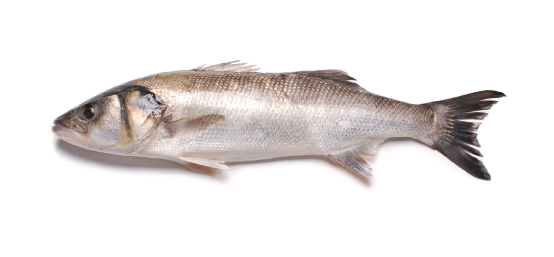
\includegraphics[width=10cm]{./Robalo.png}
		\caption{Um Robalo}
	\end{figure}

	\newpage
	\tableofcontents
	\listoffigures
	\listoftables

\end{document}